\documentclass[11pt]{article}
\usepackage[toc,page]{appendix}
\usepackage{amsmath, amssymb}
\usepackage[utf8]{inputenc}
\usepackage[T1]{fontenc}
\usepackage[style=apa,backend=biber]{biblatex}
%\usepackage{biblatex}
\addbibresource{references.bib}
\usepackage{graphicx}
\usepackage{tikz}
\usetikzlibrary{automata,positioning,shapes.geometric, arrows.meta, fit, backgrounds, calc, chains}
\graphicspath{./images/Easy_Pictures/SMR_MULT_Repackaging}%\usepackage{kpfonts}
\usepackage{float}
\usepackage[margin=1in]{geometry}
\usepackage{cancel}
\usepackage{epsfig}
\usepackage{tikz-3dplot}
\usepackage{darkmode}
\usepackage{dirtytalk}
\usepackage{longtable,booktabs,array}
\usepackage{calc} % for calculating minipage widths
\usepackage[utf8]{inputenc}
\usepackage[T1]{fontenc}
\usepackage{xcolor}
\usepackage{listings}


\usepackage{etoolbox}
\usepackage{hyperref}
\hypersetup{
 colorlinks=true,
 linkcolor=blue,
 filecolor=magenta, 
 urlcolor=cyan,
 pdftitle={Hermeneutic Calculator},
 citecolor=blue,
 }


\urlstyle{same}

\lstdefinestyle{htmlStyle}{
 language=HTML,
 basicstyle=\ttfamily\small,
 keywordstyle=\color{blue}\bfseries,
 commentstyle=\color{gray}\itshape,
 stringstyle=\color{red},
 breaklines=true,
 frame=single,
 numbers=left,
 numberstyle=\tiny\color{gray},
 columns=fullflexible,
}
\lstdefinelanguage{HTML}{
 keywords={<!DOCTYPE, html, head, title, body, h1, h2, h3, p, div, span, a, img, ul, li, table, tr, td, th, style, link, script},
 sensitive=true,
 comment=[l]{//},
 morecomment=[s]{/*}{*/},
 morestring=[b]',
 morestring=[b]"
}
\lstset{style=htmlstyle, language=html}
% Updated to explicitly pass the language option
%\lstinputlisting[style=htmlstyle, language=html]{./html/example.html}
%\usepackage{tocloft}

% Optional: define some custom colors
\definecolor{sliceRed}{RGB}{225,224,91} % matching "varyellow" from your code
\definecolor{linkYellow}{RGB}{255,215,0} % a golden yellow
\tdplotsetmaincoords{70}{110}

\title{Subtraction Strategies: Rounding and Adjusting}
\author{Compiled by Theodore M. Savich}


\begin{document}
\maketitle
\subsection*{Rounding and Adjusting}


\subsection*{Transcript}
Video from \textcite{Carpenter1999}. Strategy descriptions and curation by Amy Hackenberg. 

\begin{itemize}
\item \textbf{Teacher:} Kevin had 84 gumdrops. During the week, he ate 29 gumdrops. How many gumdrops does he have left?
\item \textbf{Kevin:} 55. 
\item \textbf{Teacher:} How'd you get 55? 
\item \textbf{Kevin:} I knew if I had 80 gumdrops and I ate 20, I knew I would have 60 gumdrops. But I had to add 4 more because it was 84 minus 20, so that would be 64. And I took away 4 more, and that would be 60. But I had to take away 5 more and that would be 55. 
\end{itemize}

\subsection*{Picture}
\begin{center}
    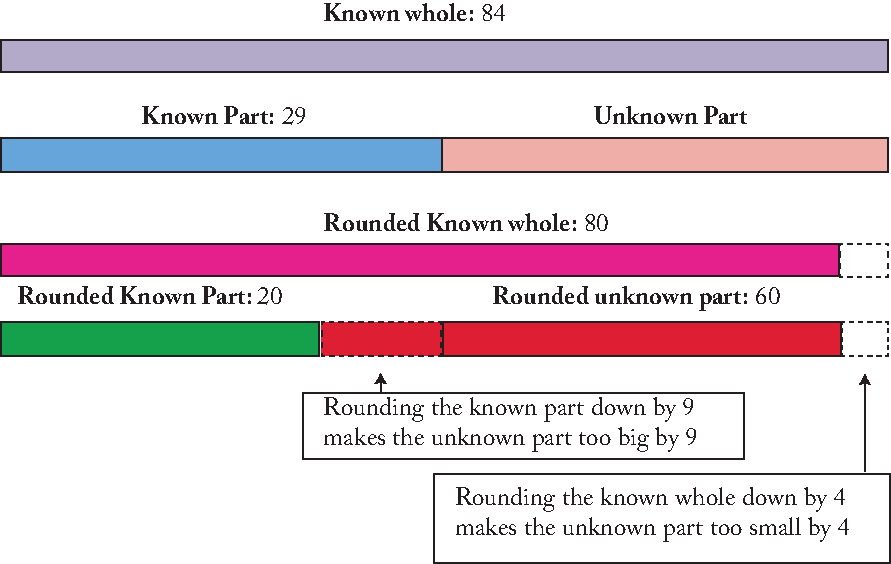
\includegraphics[width=.8\textwidth]{./images/Easy_Pictures/SAR_SUB_ROUNDING_PICTURES/PDF/SAR_SUB_Rounding.pdf}
\end{center}
\subsection*{Notation}
\textbf{Rounding}


\begin{eqnarray}
84-29 = \Box\\
84-4 = 80\\
29-9 = 20\\
80-20 = 60
\end{eqnarray}


\textbf{Adjusting}

\begin{eqnarray}
60+4 = 64\\
64-4 = 60\\
60-5 = 55
\end{eqnarray}


\subsection*{Explaining the Adjusting}
\begin{itemize}
    \item Kevin knew that if he had 80 gumdrops and ate 20, he would have 60 gumdrops left.
    \item Rounding the known whole down by 4 makes the unknown part too small by 4. 
    \item So, adjust the difference by adding 4 gumdrops back to get 64.
    \item Rounding the known part down by 9 makes the unknown part too big by 9
    \item So, adjust the difference by subtracting 9. Kevin does this by chunking back by 4 (to get 60) and then by 5 (to get 55).
\end{itemize}

\subsubsection*{Description of Strategy}
Change either the known part or the known whole to a ``good'' number—usually the nearest base—to make the subtraction easier. Then subtract and adjust your answer. This extra adjusting step can be a bit trickier than rounding when you add!
\begin{itemize}
\item If you round the known whole up, you pretend you had more than you really did, so the unknown part seems too big.
\item If you round the known whole down, you act like you had less, and you'll need to add back what you subtracted at the end. 
\item Similarly, if you round the known part down, you're not subtracting enough and must add back in. 
\item If you round the known part up, you subtract too much and need to add some back to fix it.
\end{itemize}

 







\subsubsection*{Automaton Type}
\textbf{Pushdown Automaton (PDA)}: Needed to remember the amount of adjustment required.

\subsubsection*{Formal Description of the Automaton}

We define the PDA as the 7-tuple
\[
M = (Q,\Sigma,\Gamma,\delta,q_{0/accept},Z_0,F)
\]
where:
\begin{itemize}
    \item \(Q = \{q_{0/accept},\, q_1,\, q_2,\, q_3,\, q_4\}\) is the set of states.
    \item \(\Sigma = \{0,1,2,3,4,5,6,7,8,9\}\) is the input alphabet (representing the digits of the minuend \(M\) and subtrahend \(S\)).
    \item \(\Gamma = \{Z_0\} \cup \{x \mid x \in \mathbb{Z}\}\) is the stack alphabet, where \(Z_0\) is the initial stack symbol and \(x\) represents the adjustment value.
    \item \(q_{0/accept}\) is the start state, which is also the accept state.
    \item \(F = \{q_{0/accept}\}\) is the set of accepting states.
\end{itemize}

The transition function \(\delta\) is defined by:
\begin{enumerate}
    \item \(\delta(q_{0/accept},\, \text{``}M,S\text{''},\, Z_0) = \{(q_1,\, Z_0)\}\) \\
          (Read the minuend \(M\) and subtrahend \(S\).)
    \item \(\delta(q_1,\, \varepsilon,\, Z_0) = \{(q_2,\, Z_0)\}\) \\
          (Decide which number to round and determine the rounding strategy.)
    \item \(\delta(q_2,\, \varepsilon,\, Z_0) = \{(q_3,\, a\,Z_0)\}\) \\
          (Perform the rounding. Let \(a\) be the adjustment amount where, for example, if rounding the subtrahend, \(a = S' - S\).)
    \item \(\delta(q_3,\, \varepsilon,\, a) = \{(q_4,\, a)\}\) \\
          (Compute the preliminary difference using the rounded value; that is, compute \(M - S'\).)
    \item \(\delta(q_4,\, \varepsilon,\, a) = \{(q_{0/accept},\, Z_0)\}\) \\
          (Adjust the preliminary difference by incorporating \(a\) (i.e., final difference \(= (M - S') + a\)) and output the result.)
\end{enumerate}

\subsubsection*{Automaton Diagram for Rounding and Adjusting}

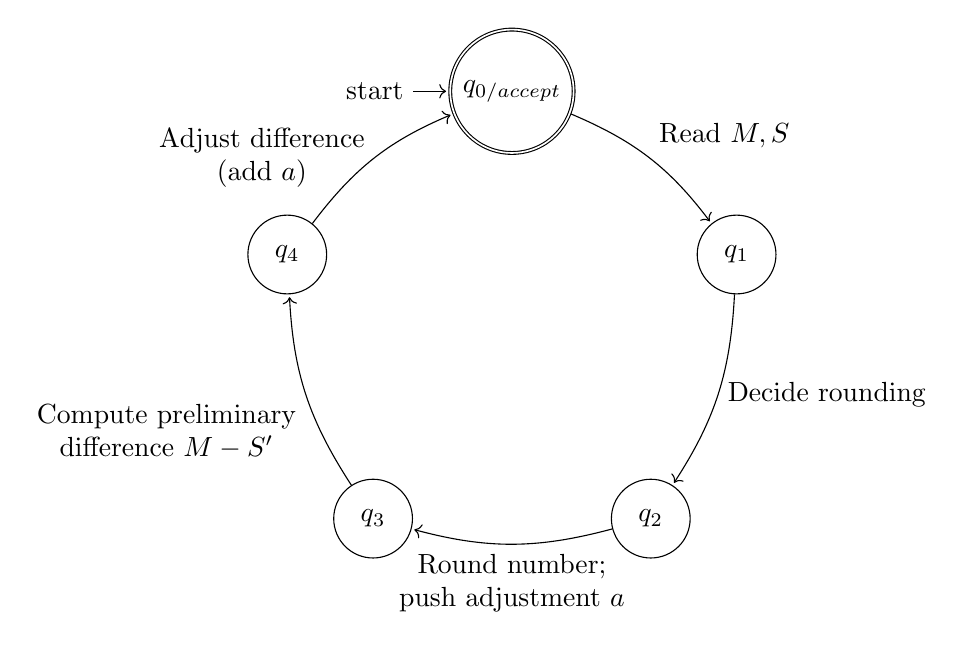
\begin{tikzpicture}[
    shorten >=1pt,
    auto,
    node distance=3cm,
    every state/.style={minimum size=1cm}
]
    % Arrange 5 states on a circle.
    \node[state, initial, accepting] (q0) at (90:3cm) {$q_{0/accept}$};
    \node[state] (q1) at (18:3cm) {$q_1$};
    \node[state] (q2) at (-54:3cm) {$q_2$};
    \node[state] (q3) at (-126:3cm) {$q_3$};
    \node[state] (q4) at (-198:3cm) {$q_4$};

    \path[->]
        (q0) edge[bend left=15] node[above right, align=center] {Read \(M,S\)} (q1)
        (q1) edge[bend left=15] node[right, align=center] {Decide rounding} (q2)
        (q2) edge[bend left=15] node[below, align=center] {Round number;\\push adjustment \(a\)} (q3)
        (q3) edge[bend left=15] node[below left, align=center] {Compute preliminary\\difference \(M-S'\)} (q4)
        (q4) edge[bend left=15] node[left, align=center] {Adjust difference\\(add \(a\))} (q0);
\end{tikzpicture}


\subsubsection*{HTML Implementation}
\lstinputlisting[style=htmlStyle, language=html]{./new_html/SAR_SUB_Rounding.html}

\end{document}